\newpage
\chapter{Евристични алгоритми}
\label{chapter02}

Евристичните алгоритми са подход за решаване на изчислителни проблеми, основаващи се на опита и интуицията. Този вид алгоритми не гарантират оптимално решение за поставената задача. Евристичните алгоритми намират широко приложение при задачи, които трудно се поддават на точни числени методи или аналитични решения. Макар и да не могат да предложат оптимално решение, евристичните алгоритми\index{евристични алгоритми} често водят до достатъчно приемливи в практиката, близки до оптималното решения. Благодарение на своята не детерминистична природа, евристичните алгоритми\index{евристични алгоритми} са изключително подходящи за реализация в супер компютърни изчисления\index{супер компютърни изчисления}. Две изключително популярни евристики\index{евристики} са изкуствените невронни мрежи\index{изкуствени невронни мрежи} и генетичните алгоритми\index{генетични алгоритми}. Те са обект на особена популярност през последните две десетилетия и това дава основание да бъдат заложени в основното изложение на настоящото учебно помагало. Сами по себе си евристиките са безполезни, ако не бъдат приложени върху достатъчно сложна изчислителна задача. Точно такава сложност предлагат задачите за прогнозиране. Прогнозирането е залегнало в множество дейности от човешкото ежедневие като започнем от средните дневни температури и стигнем до потреблението на определени стоки и услуги. Под една или друга форма почти всяка човешка дейност бива остойностена в термините на финансовите ресурси. Този факт дава основание да бъдат разгледани точно прогнози за промяната в цените на различни финансови инструменти. Отчитането на промяната в цената на определени интервали (равни или неравни) води до представяне на информацията във времеви ред\index{времеви редове}. При времевите редове\index{времеви редове} по абсцисната ос се означава времето, а по ординатната ос стойността на измерваната величина (в конкретния случай цената).

\section{Финансови времеви редове}

Времевите редове\index{времеви редове} са серия от замервания извършени в последователен ред във времето. Практически се получава последователност от дискретни стойности. Времевите редове могат да са съставени от стойности на равни интервали или стойности на произволни интервали. Често в практиката се случва да има липсващи замервания, което води до определени усложнения при анализирането. При финансовите времеви редове основно се използват равни интервали на отчитане и рядко има липсващи стойности при отчитането. Всяко едно отчитане при финансовите времеви редове се отличава с група стойности, характеризиращи времевия интервал за който се отнася, а именно – начална стойност за интервала, най-висока постигната стойност за интервала, най-ниска стойност постигната за интервала и крайна стройност за интервала. 

\begin{figure}[h]
  \centering
  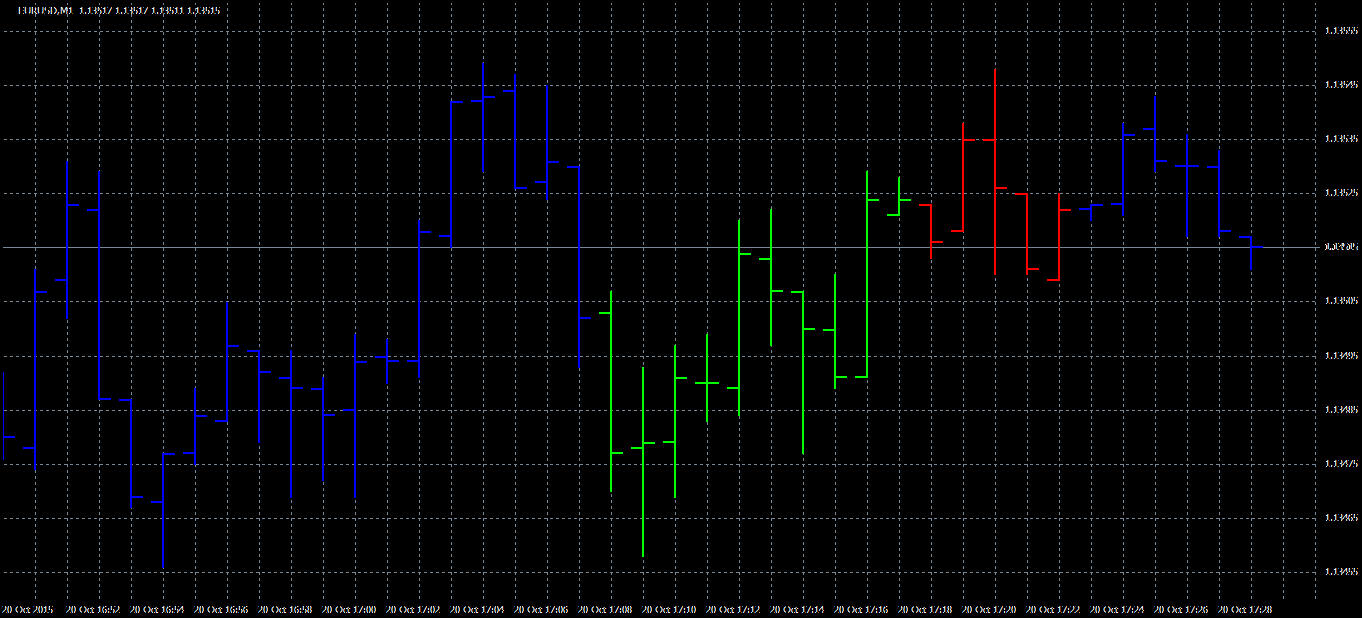
\includegraphics[width=1.0\linewidth]{pic0003}
  \caption{Отношението евро/долар в рамките на един час}
\label{fig:pic0003}
\end{figure}

На Фиг. \ref{fig:pic0003} тази информация се обозначава с вертикални черти, като долният край на вертикалната черта символизира най-ниското ниво, горният край най-високото ниво, а двете странични чертички маркират нивото на отваряне (отляво) и нивото на затваряне (от дясно). Анализирането на времевите редове\index{времеви редове} може да предостави съществена информация за лицата вземащи решения. Когато става въпрос за времеви редове във финансовата област основна цел на анализа е предлагането на прогноза. Една от най-често използваните форми на анализ е напасването на крива (curve fitting). От математическа гледна точка задачата представлява построяване на крива която да премине максимално близо до предварително определени точки. От математиката е добре известно, че през краен брой точки могат да се построят безкрайно на брой преминаващи криви. За да има смисъл от напасването кривата трябва да притежава определени свойства като изглаждане, добра интерполация и екстраполация. 

Условното разделяне на финансовия времеви ред\index{финансови времеви редове} на две половини (минало и бъдеще) дава изключително добра възможност за представяне на задачата по прогнозиране в термините на изкуствените невронни мрежи\index{изкуствени невронни мрежи}. Мащабираната информация от миналия период (зелено на графиката) се подава към входния слой на изкуствената невронна мрежа, а прогнозата се получава в изходния слой на изкуствената невронна мрежа и се подлага на обратно мащабиране (червеното на графиката). Така декомпозиран времевият ред\index{времеви редове} се използва при фазата за обучение на изкуствената невронна мрежа. За работната фаза на мрежата за прогноза на изкуствената невронна мрежа се подават последните измерени стойности, без да има яснота какви са бъдещите измервания. 

\section{Изкуствени невронни мрежи}

Изкуствените невронни мрежи\index{изкуствени невронни мрежи} са се появили в следствие на опитите за изграждане на математически модел за биологичните нервни системи. Този вид системи се научават (прогресивно подобряват възможностите си) с изследването на примерни данни. Приложението им е основно при задачи, за които традиционните алгоритми не дават приемливи резултати. Най-широко приложение изкуствените невронни мрежи намират в задачи за класификация. Когато става въпрос за финансови времеви редове, са възможни две събития – повишаване на стойността или понижаване на стойността. Според информацията в отминалите периоди време, изкуствената невронна мрежа\index{изкуствени невронни мрежи} може да раздели данните в два основни класа – данни показващи промяна към повишение или данни показващи промяна към понижение. 

\begin{figure}[h]
  \centering
  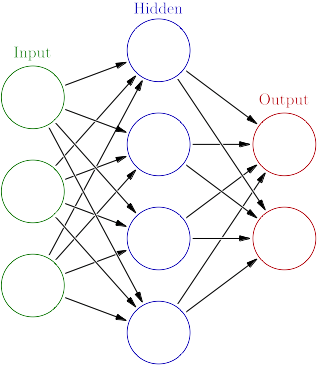
\includegraphics[height=0.25\pdfpageheight]{pic0004}
  \caption{Трислойна изкуствена невронна мрежа}
\label{fig:pic0004}
\end{figure}

Структурата на класическите изкуствени невронни мрежи\index{изкуствени невронни мрежи} се състои от възли, наречени изкуствени неврони и връзки, наречени тегла (Фиг. \ref{fig:pic0004}). Връзките между невроните служат за предаване на сигнал от един неврон към друг. Невроните които получават сигнали ги обработват по предварително заложено правило и след това могат на свой ред да ги разпространят към други неврони. В класическия случай невроните имат стойност (обикновено това е реално число). Връзките между невроните също са представени със стойност и според правилото за обучение точно тази стойност подлежи на промяна, така че мрежата да заучава необходимата информация. При най-използваните изкуствени невронни мрежи\index{изкуствени невронни мрежи} невроните са организирани в слоеве. Сигналите при този вид мрежи се разпространяват от входния слой към изходния слой, като преминават междинните слоеве. Това разпространение на сигналите се нарича пас в права посока и е характерно за режима на употреба. Освен режим на употреба изкуствените невронни мрежи\index{изкуствени невронни мрежи} работят и във втори режим, наречен режим на обучение. За последните няколко десетилетия са предложени множество начини за обучение на изкуствени невронни мрежи като най-значими резултати се получават при използването на алгоритъма за обратно разпространение на грешката\index{обратно разпространение на грешката}. Обратното разпространение на грешката представлява точен числен метод от групата на градиентните методи, който разчита на грешката, която мрежата допуска при изпълнението на обучаващите примери. Тази допусната грешка се установява в изходния слой и след това се разпространява обратно по предходните слоеве, от където идва и названието на метода. 

Според своята линейна природа, обратното разпространение на грешката\index{обратно разпространение на грешката} трудно се поддава на реализация в термините на паралелното програмиране. Ако се погледне на теглата в една изкуствена невронна мрежа като на многомерно безкрайно пространство от реални числа, то намирането на стойности за теглата е математическа оптимизационна задача. Точните числени методи дават добри резултати при пространства с относително малка размерност, но срещат сериозни затруднения при по-големите размерности. Точно противоположно на точните числени методи, евристичните алгоритми предлагат приемливи решения в разумно време. Предимство е не само ефективността, но и значително по-големите възможности евристичните алгоритми да се реализират в термините на паралелното програмиране. 

Класическите неврони реализират трансферна функция и активационна функция. Най-често използваната трансферна функция е линейната, която представлява сума от умножение на входните сигнали по теглата, които ги доставят. Най-често използваните активационни функции са сигмоидната функция и хиперболичният тангенс. Активационната функция има основна роля за нормиране на изходния сигнал. Тази нормализация е необходима тъй като за трансферната функция при различните неврони постъпват различен брой сигнали и без нормализация това би направило изходните сигнали несъизмерими. При градиентните точни числени методи има изискване активационната функция да бъде диференцируема, нещо което не е необходимо при евристичните алгоритми. Често използваната линейна трансферна функция има нужда от използване на допълнително събираемо наречено „отместване“ (bias). От формална гледна точка, отместването може да се интерпретира като тегло свързващо неврона с друг неврон, който емитира единичен сигнал. В практиката за всеки слой е прието да се отделя неврон емитиращ единичен сигнал. Само в изходния слой е безсмислено такъв неврон да има, тъй като той не получава входни сигнали, а емитирането на постоянна единица в изхода не носи смислена информация за функционирането на мрежата. 

От математическа гледна точка класическите невронни мрежи могат да се представят с вектор (стойностите на невроните) и матрица (стойностите на теглата между невроните). Разпространението на сигналите от входа към изхода в този случай би бил умножение на вектор с число. В настоящото учебно помагало на класическа трислойна мрежа ще се подават мащабираните стойности от изминалите времеви периоди, а на изхода ще се очаква прогнозна стойност за бъдещи времеви интервали. Тази концепция е малко по-сложна от идеята за проста квалификация от вида повишение/понижение, но е значително по-информативна, защото се очаква да дава представа за един по-дълъг времеви интервал в бъдещето. След успешно прогнозиране в коя посока ще се промени цената от съществено значение става и въпросът колко дълго ще продължи този спад/повишение. 

\section{Генетични алгоритми}

Генетичните алгоритми са глобална оптимизационна евристика\index{глобална оптимизационна евристика} вдъхновена от идеите за биологичната еволюция. Генетичните алгоритми са подмножество на класовете популационни алгоритми и еволюционни алгоритми. Основното си приложение генетичните алгоритми\index{генетични алгоритми} намират при задачи с голямо по размерност пространство на решенията. Често при такива задачи класическите точни числени методи не могат да предложат решение в приемливо време. За да се приложи генетичен алгоритъм, решението на съответната задача трябва да се представи под формата на хромозома (индивид) в обща популация от решения. След това, чрез прилагане на основните операции по селекция\index{селекция в генетичен алгоритъм}, кръстосване\index{кръстосване в генетичен алгоритъм} и мутация\index{мутация в генетичен алгоритъм} (Фиг. \ref{fig:pic0005}), отделните индивиди (решения) следва да бъдат подобрявани.

\begin{figure}[h]
  \centering
  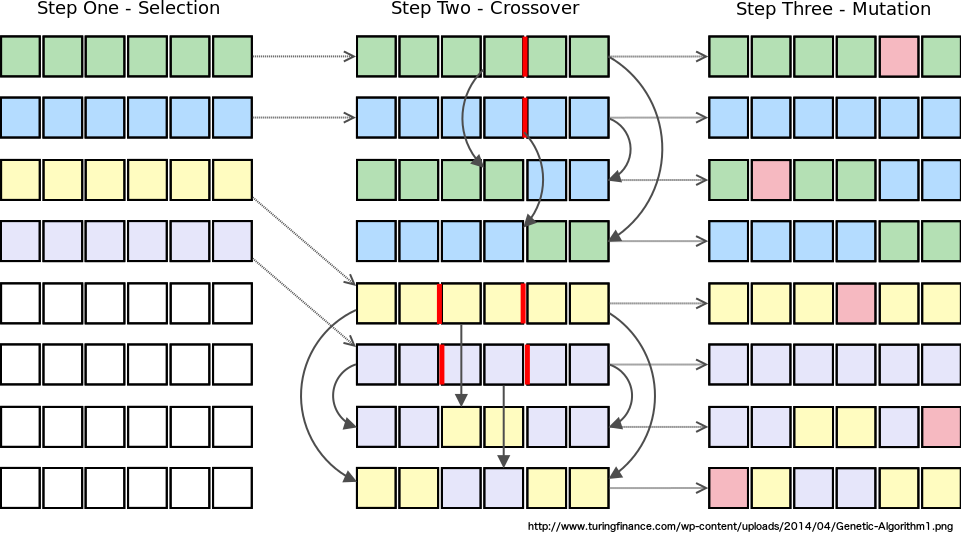
\includegraphics[width=1.0\linewidth]{pic0005}
  \caption{Трите основни операции в генетичните алгоритми}
\label{fig:pic0005}
\end{figure}

При класическия процес оптимизацията започва от случайно генерирани индивиди. Това не е задължително, особено когато става въпрос за хибридни реализации, в които генетичният алгоритъм е поддържаща оптимизация. При такива ситуации началната популация може да бъде получена в резултат на друга оптимизация или в резултат на човешка подредба. След началната фаза оптимизацията протича итеративно и приключва според предварително определени критерии за край. Най-често се използва предварително дефиниран брой поколения или брой поколения, които не водят до подобрение в намерените решения, но също така е възможно да се дефинира и интервал астрономическо време. 

От основна важност за успешната работа с генетичните алгоритми\index{генетични алгоритми} е определянето на целева функция (жизнена функция\index{жизнена функция} на индивида), която еднозначно да определя качеството на полученото решение. На база различната жизненост която индивидите в популацията притежават, се взема стохастично решение кои индивиди да участват в създаването на бъдещото поколение и кои не. В множество реализации на генетични алгоритми се прилага правило на елита, така че най-доброто открито решение да достигне края на оптимизационния процес. В същото време правилото на елита крие риск от израждане на популацията, така че всичките решения в нея да клонят към съхранения елит.  

Фактът, че генетичните алгоритми са организирани на принципа на популацията от индивиди, ясно подсказва идеалната възможност оптимизационният процес да се организира не в една глобална популация, а в множество различни локални популации, които да съществуват на различни изчислителни машини. Това от своя страна би дало възможност за реализиране на миграционни процеси, точно както това се наблюдава при естествените биологични видове. 

\section{Прогнозиране в разпределена среда}

Гъвкавите възможности на изкуствените невронни мрежи\index{изкуствени невронни мрежи} да изграждат функционална зависимост между входни и изходни данни ги прави идеален кандидат за прогнозираща система. Ако се приеме, че измерените стойности във времевия ред са точки в двуизмерно пространство, то задачата за прогнозиране може да се представи като задача за прекарване на крива през N точки (curve fitting). Ако образно се оприличи изкуствената невронна мрежа на полином, то теглата й биха представлявали коефициенти в полинома. Стойностите които изкуствената невронна мрежа\index{изкуствени невронни мрежи} генерира на изхода си за бъдещи моменти от времето, са своеобразна екстраполация\index{екстраполация} според апроксимираната крива. Тъй като класическите многослойни невронни мрежи работят с входни сигнали между 0.0 и 1.0 или -1.0 и +1.0, то информацията от времевия ред трябва да бъде мащабирана в съответния работен интервал на мрежата. Стойностите на времевия ред условно се разделят на минали (зелените Фиг. \ref{fig:pic0003}) и бъдещи (червените Фиг. \ref{fig:pic0003}). Изходната (прогнозна) информация на изкуствената невронна мрежа след това се мащабира обратно към оригиналните интервали на времевия ред.

\begin{figure}[h]
  \centering
  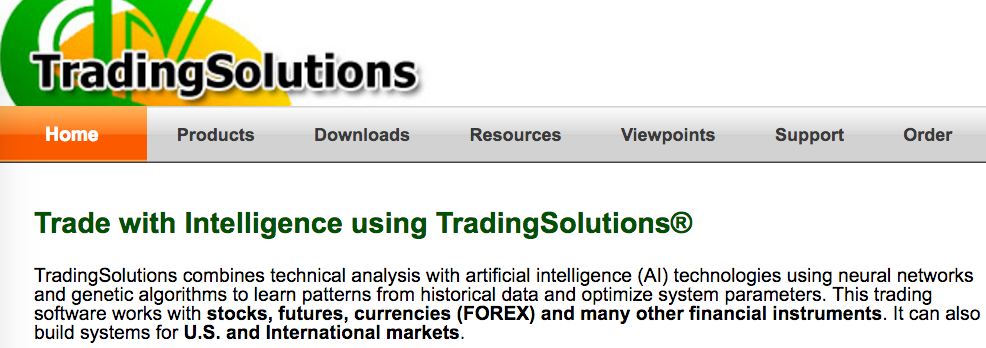
\includegraphics[width=1.0\linewidth]{pic0006}
  \caption{Продуктовата линия TradingSolutions използваща изкуствени невронни мрежи и генетични алгоритми за прогнозиране на Forex финансови инструменти}
\label{fig:pic0006}
\end{figure}

От чисто практическа гледна точка, използването на изкуствени невронни мрежи и генетични алгоритми се е доказало като удачен подхода за прогнозиране на финансови инструменти, което ясно се вижда в продуктовата линия на TradingSolutions (Фиг. \ref{fig:pic0006}). Почти петнадесет години продуктовата линия на TradingSolutions доставяше системи за подпомагане вземането на решения\index{системи за подпомагане вземането на решения}. По настоящем, тази продуктова линия е придобита от компанията nDimensional, Inc.

\begin{figure}[h]
  \centering
  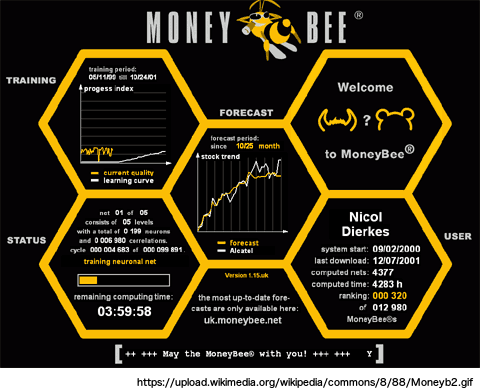
\includegraphics[height=0.4\pdfpageheight]{pic0007}
  \caption{Системата MoneyBee за финансово прогнозиране в разпределена среда}
\label{fig:pic0007}
\end{figure}

Възможността да се прогнозират цените на финансови инструменти винаги е привличала не само индустрията, но и научните среди. Едно от най-забележителните постижения в тази насока е проектът MoneyBee (Фиг. \ref{fig:pic0007}). Макар и вече да не съществува, този проект предлагаше възможност за изчисляване на прогнози с помощта на дарена изчислителна мощност\index{дарени изчислителни ресурси} в разпределена среда\index{изчисления в разпределена среда} \cite{bohn}. Същинските прогнози се пресмятаха, с помощта на изкуствени невронни мрежи, върху изчислителните машини на потребителите в периоди когато натоварването на машините е ниско и се активира програмата за защита на монитора (screensaver). Преди масовото навлизане на мобилните устройства честа практика при проектите за дарена изчислителна мощност с цел пресмятане в разпределена среда\index{изчисления в разпределена среда}, основен подход бе извършване на пресмятанията в специално създадена за целта програма за предпазване на монитора. След навлизането на катодно лъчевите тръби при настолните компютри се появява ефект от увреждане на монитора, ако върху него продължително се визуализира статична картина. Решаването на този проблем се оказва най-удачно с помощта на операционната система, която да установи период в който потребителят не използва изчислителната машина и да активира софтуерна програма за предпазване на монитора. Развитието на мониторите с течни кристали постепенно изведе от употреба мониторите с катодно-лъчеви тръби и използването на програми за предпазване на монитора изгуби своето първоначално предназначение. Въпреки това този вид софтуерни решения останаха в употреба и основно служат за повишаване на информационната сигурност, като не само дават естетическа визуализация, но и привеждат работната сесия на потребителя в заключено състояние, което възпрепятства използването на компютърната система от неоторизирани потребители. Наличието на изчислителни ресурси, които са неефективно използвани, дава основание на множество учени да разработят системи за отдалечено пресмятане в разпределена среда\index{изчисления в разпределена среда} точно под формата на програми за предпазване на монитора, които да се възползват от дарените потребителски изчислителни ресурси. 

\section{Фонови пресмятания върху мобилни устройства}

Съществува концептуална разлика в начина, по който потребителите използват настолните си компютри и мобилните устройства. На първо място, настолният компютър бива пускан и спиран според нуждите на потребителя, докато най-често мобилните устройства са в непрекъснат режим на употреба. Това води до основната разлика, че мобилните устройства не изпадат в режим на занижена употреба, но също така имат режими за употреба при изключителна важност (примерно телефонно обаждане с висок приоритет). Втората фундаментална разлика се състои във факта, че основен похват за пестене на електрическа енергия, доставяна предимно от батерии при мобилните устройства, е динамичното изгасване на екрана. Тази стратегия за пестене на енергия кардинално отменя концепцията за програма, предпазваща монитора. За да се реализира ефективно система за разпределени пресмятания върху мобилни устройства, е много по-удачно да се използва технологията за активен тапет, отколкото да се залага на идеята за програма, предпазваща монитора. Точно тази идея е развита в настоящото учебно помагало.